Em uma das reuniões com nossos orientadores, percebemos que com poucas primitivas - objetos simples como círculos, triângulos e retângulos - e com algumas propriedades físicas configuráveis poderíamos gerar uma grande quantidade de cenários diferentes entre si. Tais propriedades, como massa, gravidade, coeficiente de atrito e de elasticidade, já eram do nosso domínio de conhecimento pois as utilizamos ao implementar os cenários de demonstração. \\

O Physimulation é o resultado dessa ideia e é o principal produto do nosso trabalho.

\subsection{A ferramenta}
Com o Physimulation o usuário pode criar quatro tipos de objetos: círculos, triângulos, retângulos e segmentos, em qualquer posição da tela. Cada tipo de objeto possui algumas propriedades específicas à sua forma. Por exemplo, o círculo é a única das primitivas que possui o atributo ''raio''. Porém, a grande maioria dos parâmetros são comuns a todas as formas:

\begin{itemize}
	\item Posição;
	\item Massa;
	\item Momento de Inércia;
	\item Coeficiente de Atrito;
	\item Coeficiente de Elasticidade;
	\item entre outros.
\end{itemize} 

Ao posicionar o \textit{mouse} nos campos editáveis são exibidas ao usuário as descrições de cada propriedade. Além disso, para cada atributo há um valor pré-definido por padrão, caso o aluno ou professor não esteja interessado em determinar seu valor.\\

Além de determinar as propriedades de cada objeto, há a possibilidade do usuário configurar paramêtros do próprio ambiente de simulação. Tais propriedades são:

\begin{itemize}
	\item Gravidade: um vetor na forma (x, y) representando a gravidade do espaço;
	\item Coeficiente de Amortecimento: porcentagem que representa a velocidade final de um objeto em relação a velocidade inicial, em um passo da simulação. Por exemplo: com um amortecimento de valor 0.9, todos os objetos perderão 10\% de suas velocidades a cada passo da simulação;
	\item Gravitação Pontual: se for selecionada, o simulador irá considerar a atração gravitacional entre os objetos da tela. Útil para criar cenários com movimentos orbitais;
	\item Espaço Limitado: se for selecionada, o simulador irá construir quatro segmentos que limitarão o espaço da simulação para o espaço visível da tela.
\end{itemize} 

Para cada tipo de objeto há um campo ''quantidade'', que informa ao simulador o número de objetos do tipo escolhido. Este campo deve ser preenchido antes da criação dos objetos físicos e pode ser alterado posteriormente.

\begin{figure}[H]
	\centering
	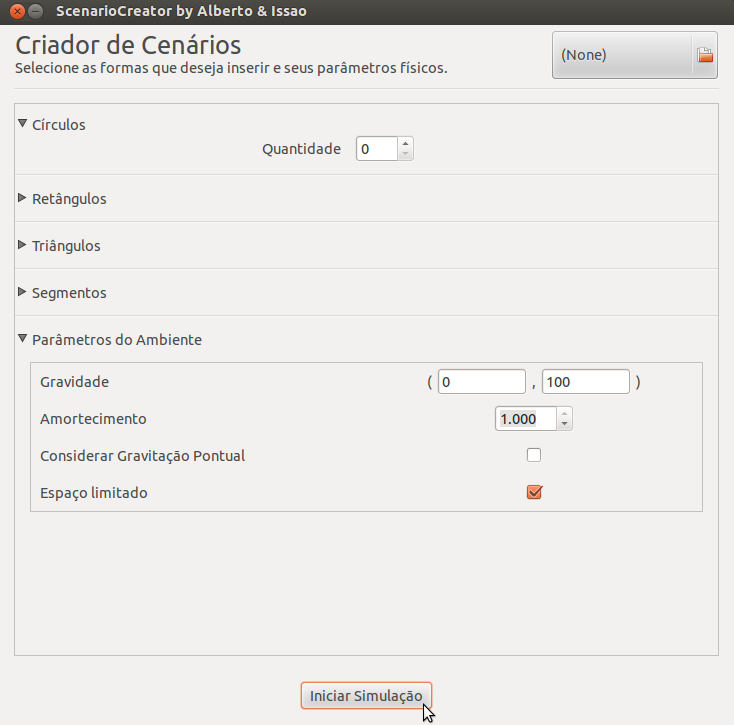
\includegraphics[scale=0.4]{images/physimulation-2.png}
	\caption{Tela inicial do Physimulation}
\end{figure}

\subsection{Criando um cenário}
Para mostrar um caso de uso do simulador, vamos utilizar a figura abaixo como referência para criar um cenário físico.

\begin{figure}[H]
  \centering
  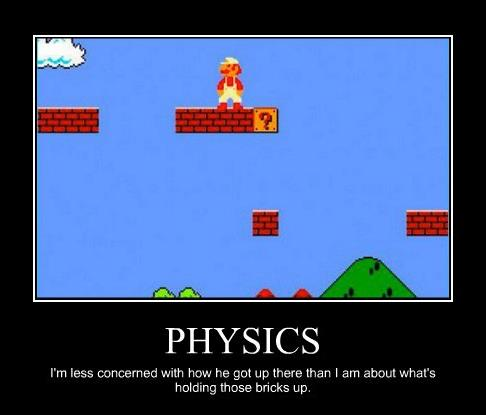
\includegraphics[scale=0.6]{images/bricks.jpg}
  \caption{Objetos estáticos \protect\cite{mario:physics}}
\end{figure}

Nesta imagem, há quatro blocos suspensos no ar e uma montanha verde com o formato parecido com um triângulo, além do personagem principal que está em cima de um dos blocos. Para esta simulação, faremos a seguinte correlação: os blocos suspensos serão retângulos do Physimulation, a montanha verde um triângulo e o personagem de pé uma pequena bola. \\

Para executar o physimulation, o usuário deve executar no terminal:

\begin{Verbatim}[fontsize=\footnotesize]
	$ cd <<DIR_PHYSIMULATION>>/Simulation
	$ ruby main.rb
\end{Verbatim}

\noindent onde {\tt\footnotesize DIR\_PHYSIMULATION} é o diretório em que o Physimulation foi instalado. Novamente, caso haja algum problema ao executar qualquer um dos comandos, deve-se verificar o conteúdo da seção \ref{instalacao}, ''\nameref{instalacao}''. \\

A seguir descrevemos os passos para criar este cenário:

\begin{enumerate}
	\item Expandir a aba ''Círculos'' e aumentar a quantidade para 1.
	\item Determinar a posição do círculo = (350, 100), massa = 30, raio = 30. \newline 
		  Nota: a origem das coordenadas no Physimulation é o canto superior esquerdo, com coordenadas positivas aquelas abaixo e à direita da origem.
	\item Expandir a aba ''Retângulos'' e aumentar a quantidade para 4.
	\item Preencher os atributos dos retângulos com os seguintes valores:
		\subitem 1º: posição = ( 80, 200), altura =  60, largura = 120 
		\subitem 2º: posição = (350, 200), altura =  60, largura = 160
		\subitem 3º: posição = (400, 400), altura =  60, largura =  60
		\subitem 4º: posição = (720, 400), altura = 120, largura =  60

	\item Em todos os retângulos anteriores, habilitar a opção ''Fixo no espaço?''. \newline 
		  Nota: ao habilitar esta opção, utilizaremos \textit{static shapes} ao invés de \textit{shapes} habituais. Na prática, estamos informando ao simulador que estes objetos não devem sofrer forças do ambiente físico (\textit{space}), como a gravidade. Para mais detalhes, ver a seção \ref{plataforma}. 

	\item Por último, criar um triângulo com os seguintes atributos: posição = (600, 520), ponto A = (100, 0), ponto B = (0, 100), ponto C = (200, 100). \newline 

\end{enumerate}

Ao iniciar a simulação, temos este cenário:

\begin{figure}[H]
	\centering
	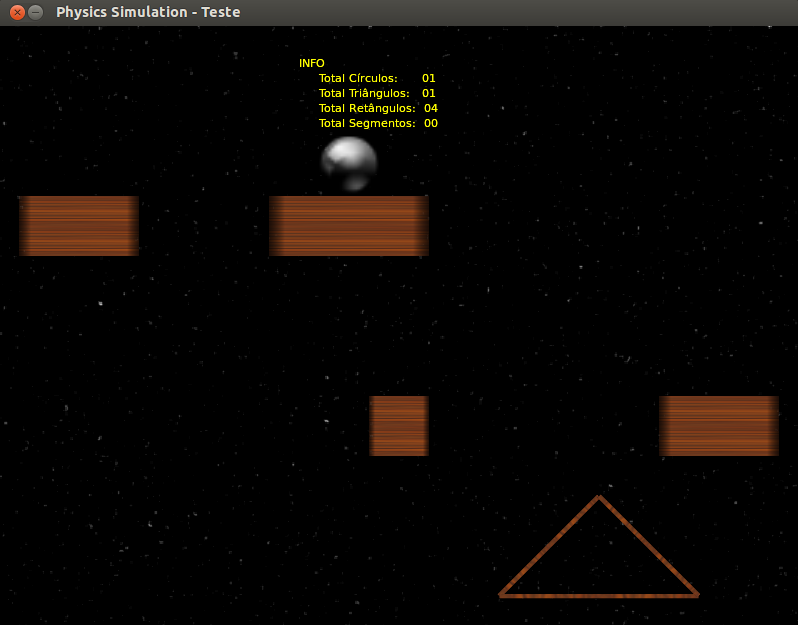
\includegraphics[scale=0.2]{images/cenario-monografia.png}
	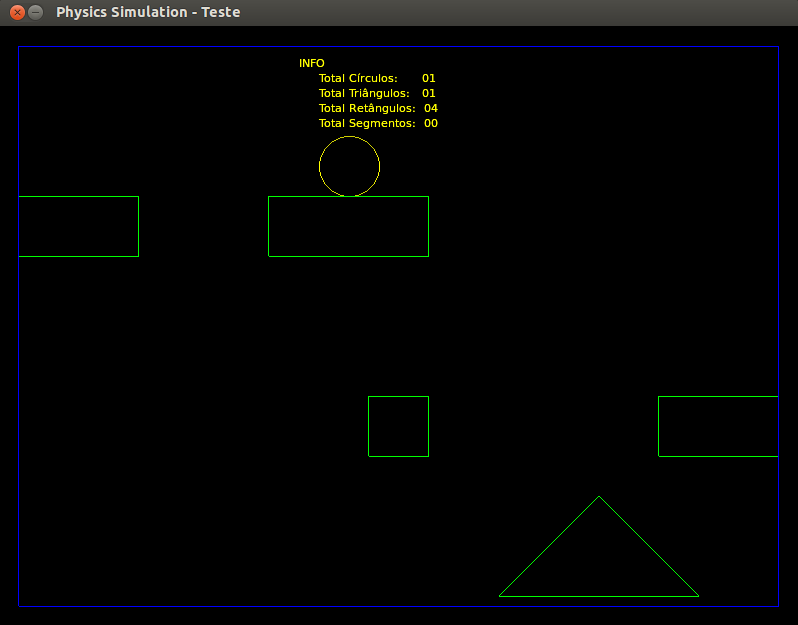
\includegraphics[scale=0.2]{images/cenario-monografiaE.png}
	\caption{Cenário criado com o Phisimulation}
\end{figure}

Podemos fazer uma pequena modificação a este cenário e acrescentar uma velocidade horizontal positiva à bola, o que a fará despencar do bloco superior. 

\begin{figure}[H]
	\centering
	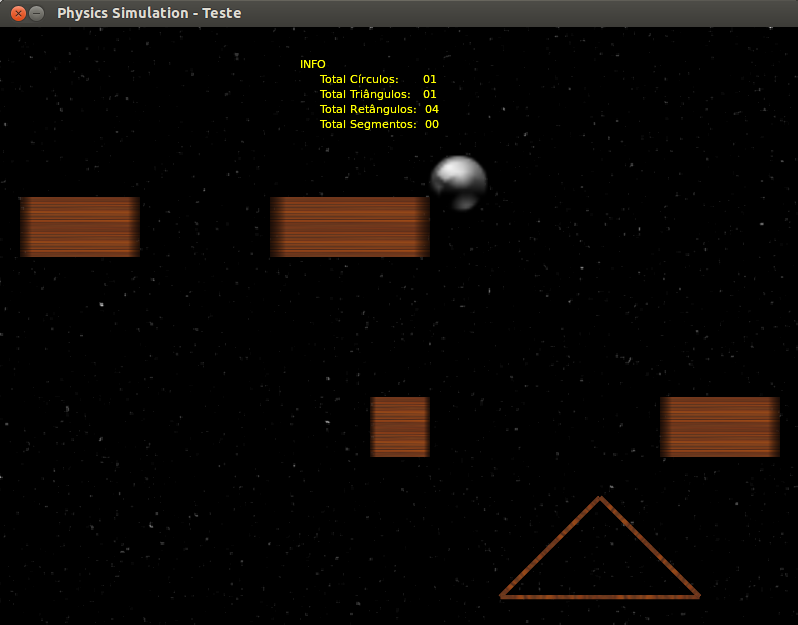
\includegraphics[scale=0.2]{images/cenario-mono-2.png}
	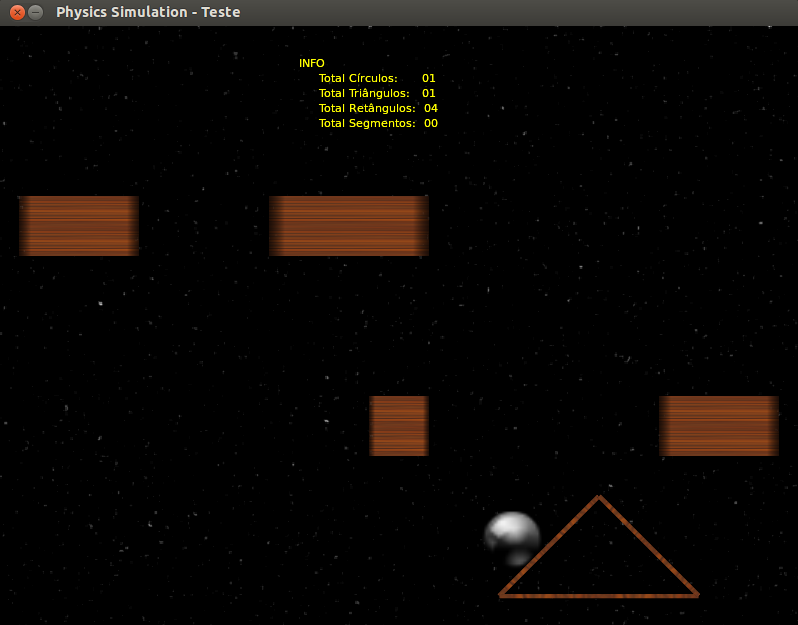
\includegraphics[scale=0.2]{images/cenario-mono-3.png}
	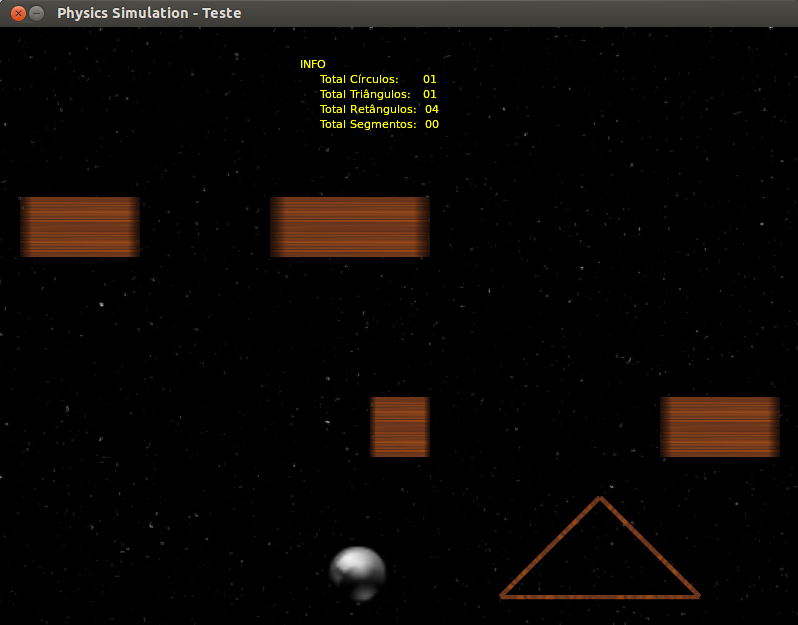
\includegraphics[scale=0.2]{images/cenario-mono-4.png}
	\caption{Mesmo cenário adicionando velocidade à bola}
\end{figure}

Há uma outra forma de iniciar uma simulação no Physimulation: utilizando um arquivo de configuração existente, com todas as propriedades dos objetos e do ambiente físico definidas. Para carregar um cenário, é necessário que o usuário use o botão no canto superior direito da interface, como mostrado na figura abaixo. \\

\begin{figure}[H]
	\centering
	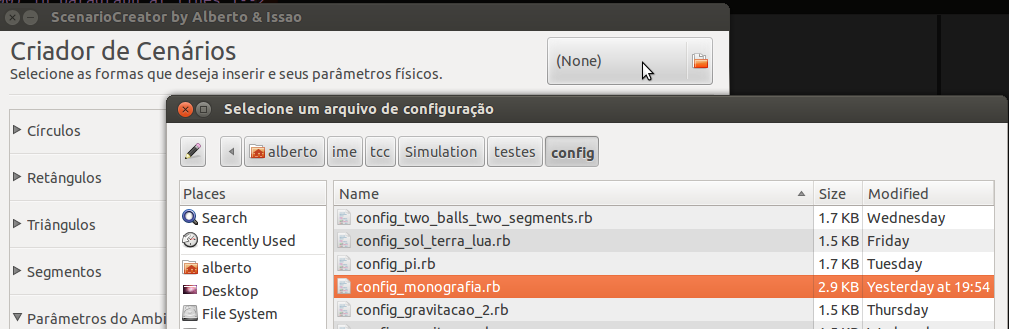
\includegraphics[scale=0.4]{images/physimulation-loading.png}
	\caption{Carregando cenários}
\end{figure}

Ao final desta seção há mais detalhes sobre o armazenamento e carregamento de cenários físicos.

\subsection{Outros exemplos}

Para o aluno ou professor que deseje aprofundar seus conhecimentos sobre a ferramenta, recomendamos a realização de vários testes com o mesmo cenário gerado, com pequenas alterações de valores entre cada teste. É importante fixar certas propriedades e observar os resultados obtidos, ao invés de modificar muitos atributos de uma só vez. \\

Abaixo há uma lista com alguns cenários criados pelo Physimulation. Todos estão disponíveis no código fonte do projeto. \\

\begin{figure}[H]
	\centering
	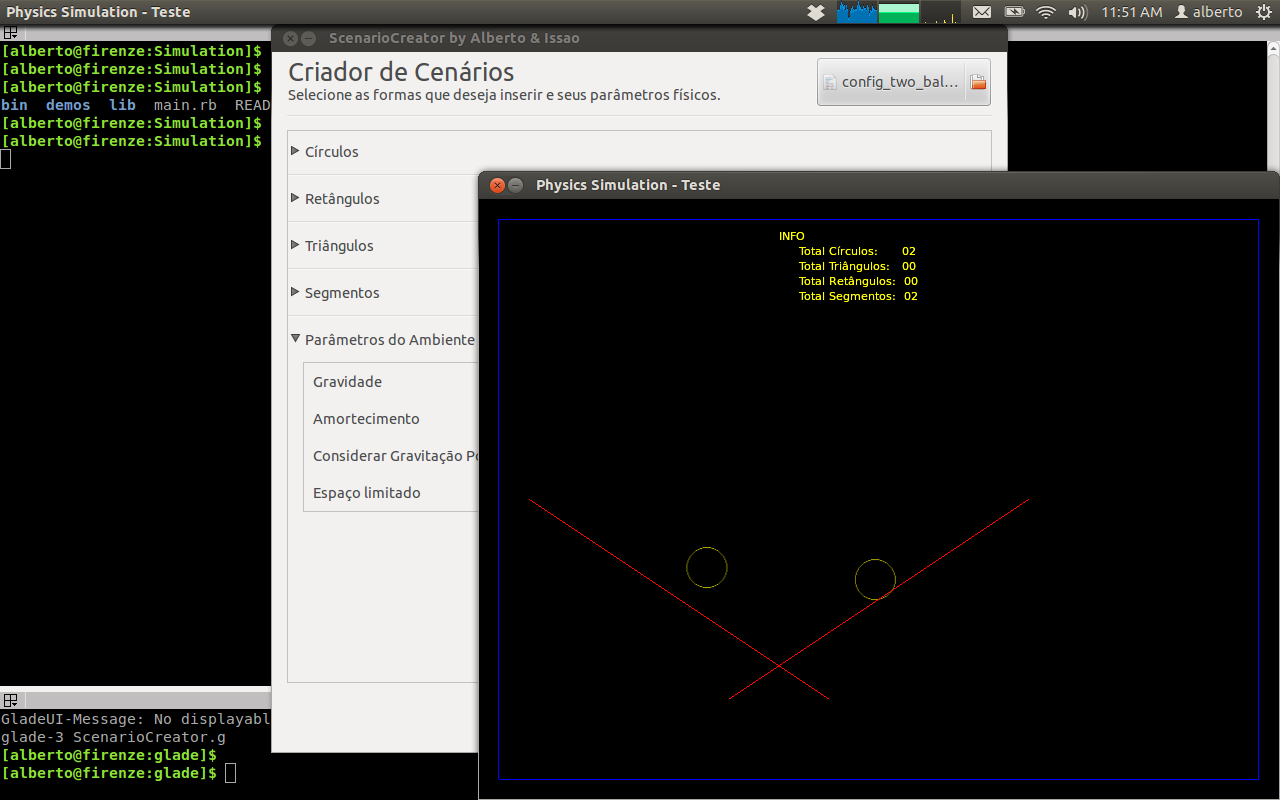
\includegraphics[scale=0.3]{images/cenario-two-balls.png}
	\caption{Cenário 1}
\end{figure}  

No cenário 1, dois segmentos são utilizados como rampa para duas bolas. Embora pareçam idênticas, a rampa da esquerda tem um coeficiente de elasticidade superior ao da direita, o que faz uma das bolas quicar para outra rampa. Já no cenário 2, abaixo, é possível observar as quatro primitivas do Physimulation, sendo que para cada tipo há um objeto fixo e outro móvel.  

\begin{figure}[H]
  \centering
  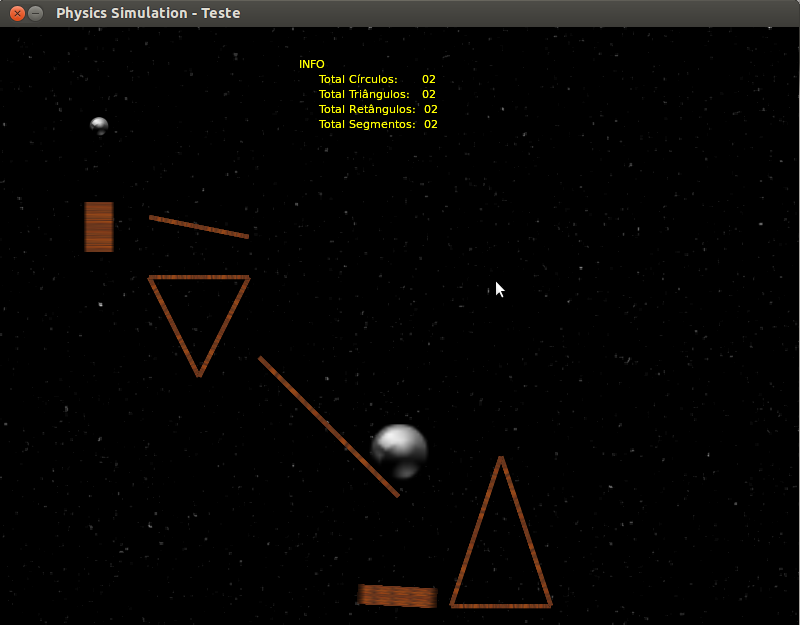
\includegraphics[scale=0.4]{images/cenario-todos.png}
\end{figure}
\begin{figure}[H]
	\centering
	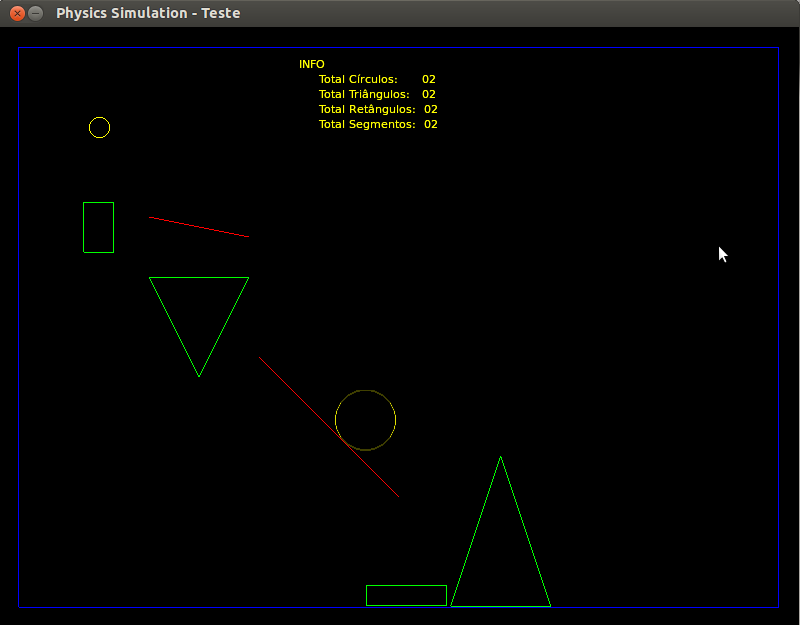
\includegraphics[scale=0.4]{images/cenario-todosE.png}
	\caption{Cenário 2}
\end{figure}

Os cenários abaixo levam em conta a atração dos corpos gravitacionais entre si e são simulações de movimentos orbitais. Para criar animações deste tipo, nosso orientador João Kerr nos sugeriu posicionar os corpos gravitacionais ao longo de um eixo imaginário; em seguida, adicionar aos corpos uma velocidade perpendicular a este eixo, variando o módulo conforme os resultados observados. Esta dica foi bastante útil para a construção destes cenários.

\begin{figure}[H]
	\centering
	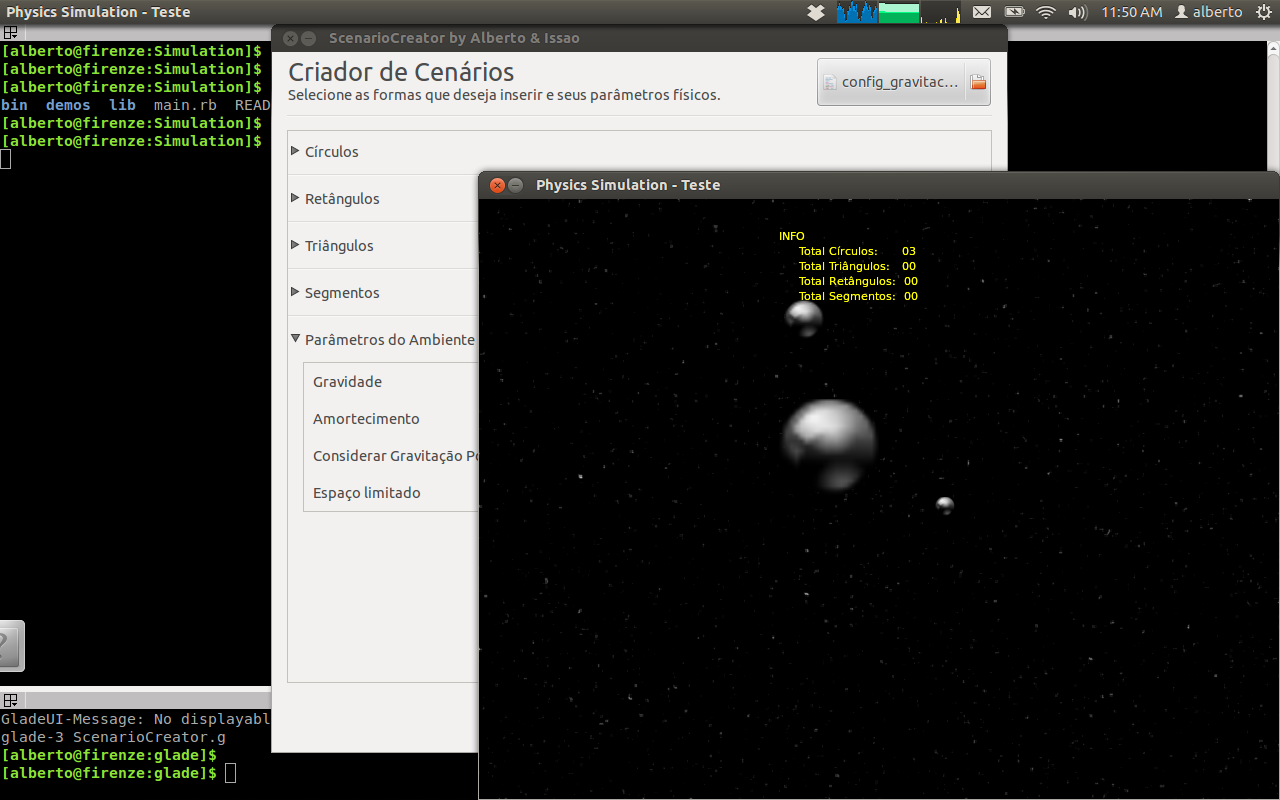
\includegraphics[scale=0.2]{images/cenario-gravitacao-2.png}
	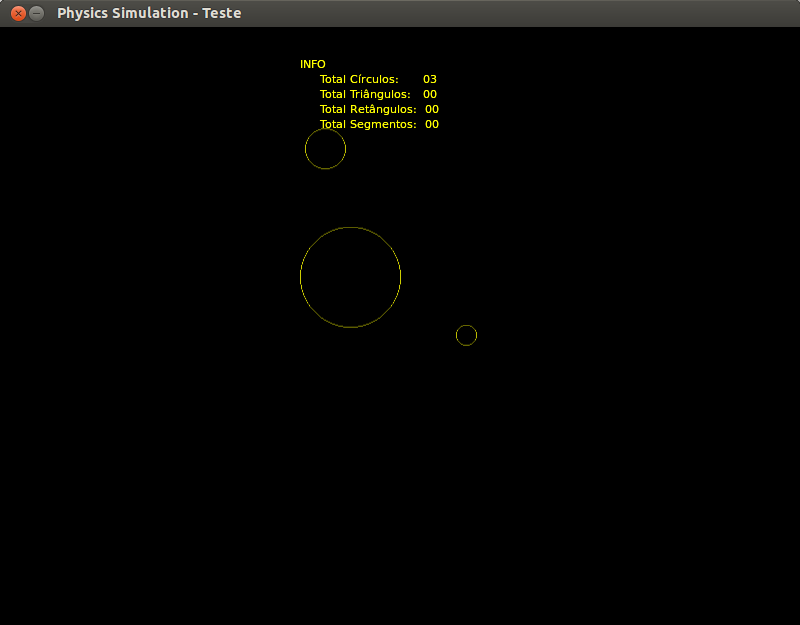
\includegraphics[scale=0.2]{images/cenario-gravitacao.png}
	\caption{Cenário com Gravitacão 1}
\end{figure}

\begin{figure}[H]
	\centering
	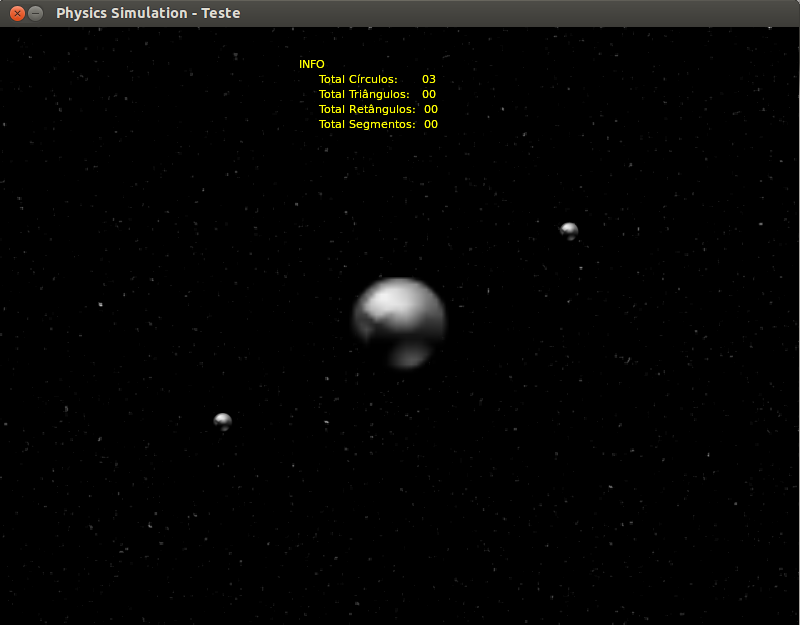
\includegraphics[scale=0.2]{images/cenario-gravitacao-4.png}
	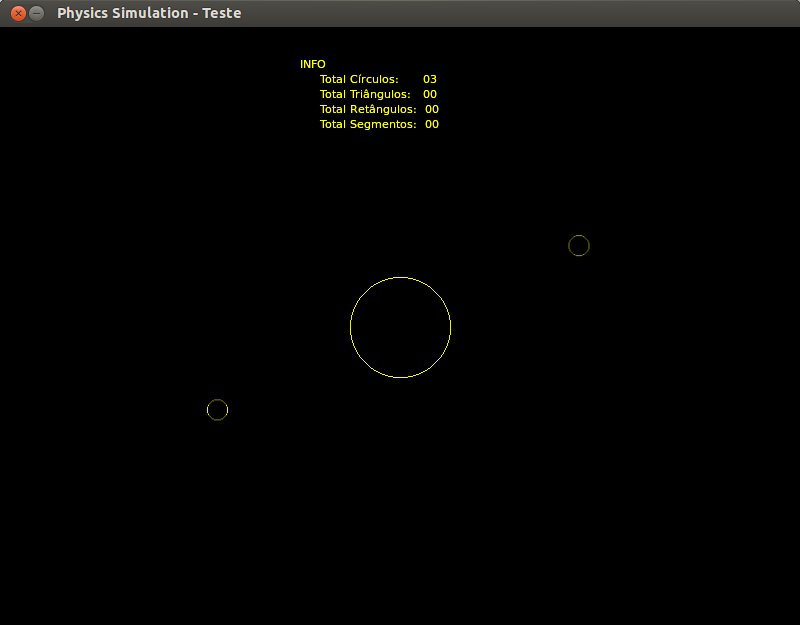
\includegraphics[scale=0.2]{images/cenario-gravitacao-3.png}
	\caption{Cenário com Gravitacão 2}
\end{figure}

No cenário a seguir há duas órbitas bem diferenciadas: das duas esferas menores em torno da maior e da esfera de menor tamanho em torno da esfera de tamanho intermediário.

\begin{figure}[H]
	\centering
	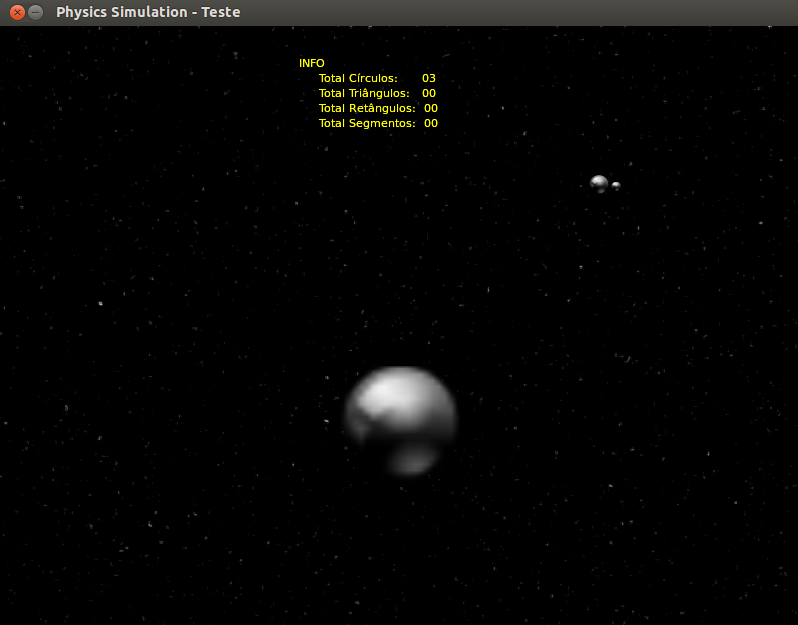
\includegraphics[scale=0.4]{images/gravitacao-sol-lua.png}
\end{figure}
\begin{figure}[H]
	\centering
	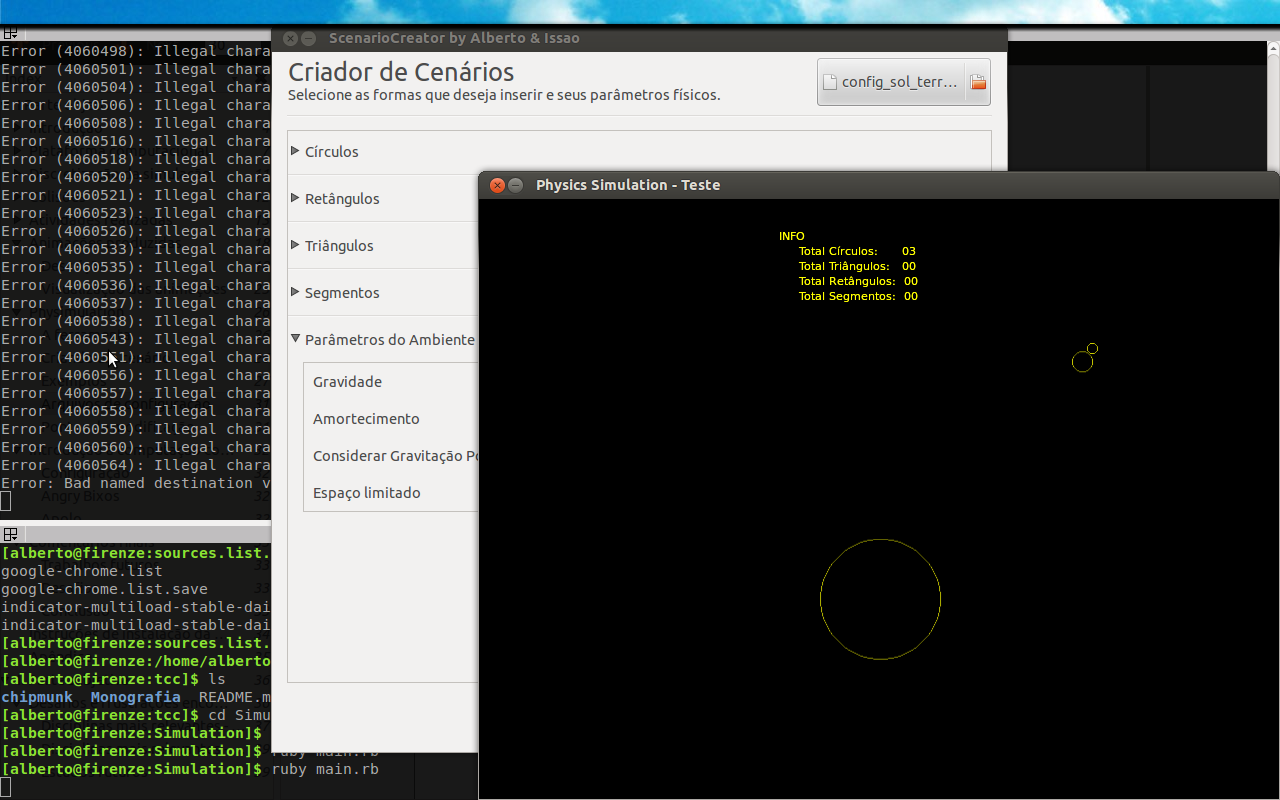
\includegraphics[scale=0.4]{images/gravitacao-sol-luaE.png}
	\caption{Cenário com Gravitacão 3}
\end{figure}

\subsection{Arquivos de configuração}
As propriedades físicas do cenário e de cada objeto ficam guardadas em um arquivo {\tt *.rb} que pode ser modificado diretamente, sem o uso do Physimulation. Observar e entender estes arquivos é importante para que o aluno do BCC entenda o funcionamento do programa como um todo. \\

O processo de animação do Physimulation divide-se basicamente em três etapas: 1) O preenchimento das propriedades físicas dos objetos no criador de cenários; 2) A geração do arquivo {\tt config\_gerado.rb}; 3) A leitura deste arquivo pela classe que irá executar de fato a simulação ({\tt Test.rb}). \\

Ao alterar o arquivo de configuração manualmente e carregá-lo pelo Physimulation, o usuário estará partindo diretamente para a terceira etapa do processo, tornando-o mais rápido. \\

Para guardar no sistema um arquivo de configuração, basta copiar o arquivo gerado para outro com um nome diferente, para que o arquivo não seja sobrescrito. Por exemplo, para guardar a última configuração utilizada em um arquivo de nome ''meu\_config.rb'', o usuário pode executar o seguinte comando:

\begin{Verbatim}[fontsize=\footnotesize]
	$ cd <<DIR_PHYSIMULATION>>/Simulation/testes/config
	$ cp config_gerado.rb meu_config.rb
\end{Verbatim}

Abaixo um exemplo de arquivo de configuração:


\begin{lstlisting}[language=Ruby, caption=Exemplo de arquivo config.rb]
module TestObjectConfig

  class Space
    attr_accessor :gravity, :damping, 
                       :limited_space, :object_gravity

    def initialize
      @gravity = vec2(0, 100)
      @damping = 1.0
      @limited_space = true
      @object_gravity = false
    end

  end

  Circles = [{
    :mass => 100.0,
    :radius => 20,
    :factor_x => 2.0, 
    :factor_y => 2.0,
    :x => 200,
    :y => 100,
    :v => vec2(0.0, 0.0),
    :moment_inertia => 100000,
    :elasticity => 1.0,
    :friction => 1.0,
    :zorder => 100,
    :collision_type => :undefined0,
    :image_name => 'cannonball2.png',
    :static => false
  }]

  Segments = [{
    :x => 200,
    :y => 400,
    :thickness => 1,
    :angle => 0.0,
    :vectors => [vec2(-150, -100), 
                    vec2(150, 100)],
    :elasticity => 1.0,
    :friction => 0.0,
    :zorder => 100,
    :collision_type => :undefined0,
    :image_name => 'catapult-b.png',
    :static => true
  }]

  Rectangles = []

  Triangles = []

  end
\end{lstlisting}

\subsection{Pontos de modificação}

O Physimulation possui pontos do código que podem ser modificados de acordo com o comportamento físico desejado, o que pode ser interessante para o aluno de computação. \\

Além de modificar o próprio código do projeto, o aluno pode também aproveitar os recursos da linguagem Ruby e adicionar métodos a classes já existentes. Por exemplo, no diretório {\tt Simulation/ext/} há o arquivo: \\

  {\tt pause\_unpause.rb.example}. \\

\noindent Ele implementa um método para a classe {\tt TesteWindow}, utilizada para executar as simulações. Caso o aluno altere o nome desse arquivo para \\

  {\tt pause\_unpause.rb} \\

\noindent , o interpretador irá reconhecer o novo método e ele já poderá ser utilizado na execução das animações. \\

Neste arquivo de exemplo, há uma implementação da função \textit{pause} para simulações, associada à tecla 'P'. Assim, renomeando este arquivo e executando qualquer uma das animações, o usuário poderá utilizar automaticamente a função \textit{pause} simplesmente apertando a tecla 'P'. \\

Baseando-se neste exemplo, o aluno de computação pode criar outros pontos de modificação no Physimulation, quando julgar apropriado.

